\documentclass[tikz,border=6pt]{standalone}
\usepackage{amsmath,amssymb}
\usepackage[T1]{fontenc}
\usepackage{lmodern}
\usetikzlibrary{arrows.meta,calc}
\definecolor{ink}{HTML}{233447}
\definecolor{blue}{HTML}{286F8E}
\definecolor{pale}{HTML}{EAF3F6}
\definecolor{amber}{HTML}{E3B25D}
\definecolor{paleamber}{HTML}{FAF1DF}
\definecolor{gray}{HTML}{DCE2E8}
\definecolor{border}{HTML}{C9D1DA}
\newcommand{\meter}[2]{%
  \draw[fill=white,draw=ink,line width=.55pt] (#1-.20,#2-.16) rectangle (#1+.20,#2+.16);
  \draw[draw=ink,line width=.45pt] (#1-.13,#2-.06) arc[start angle=170,end angle=10,radius=.13];
  \draw[-{Latex[length=1.3mm]},draw=ink,line width=.45pt] (#1,#2-.09) -- (#1+.105,#2+.08);
}
\begin{document}
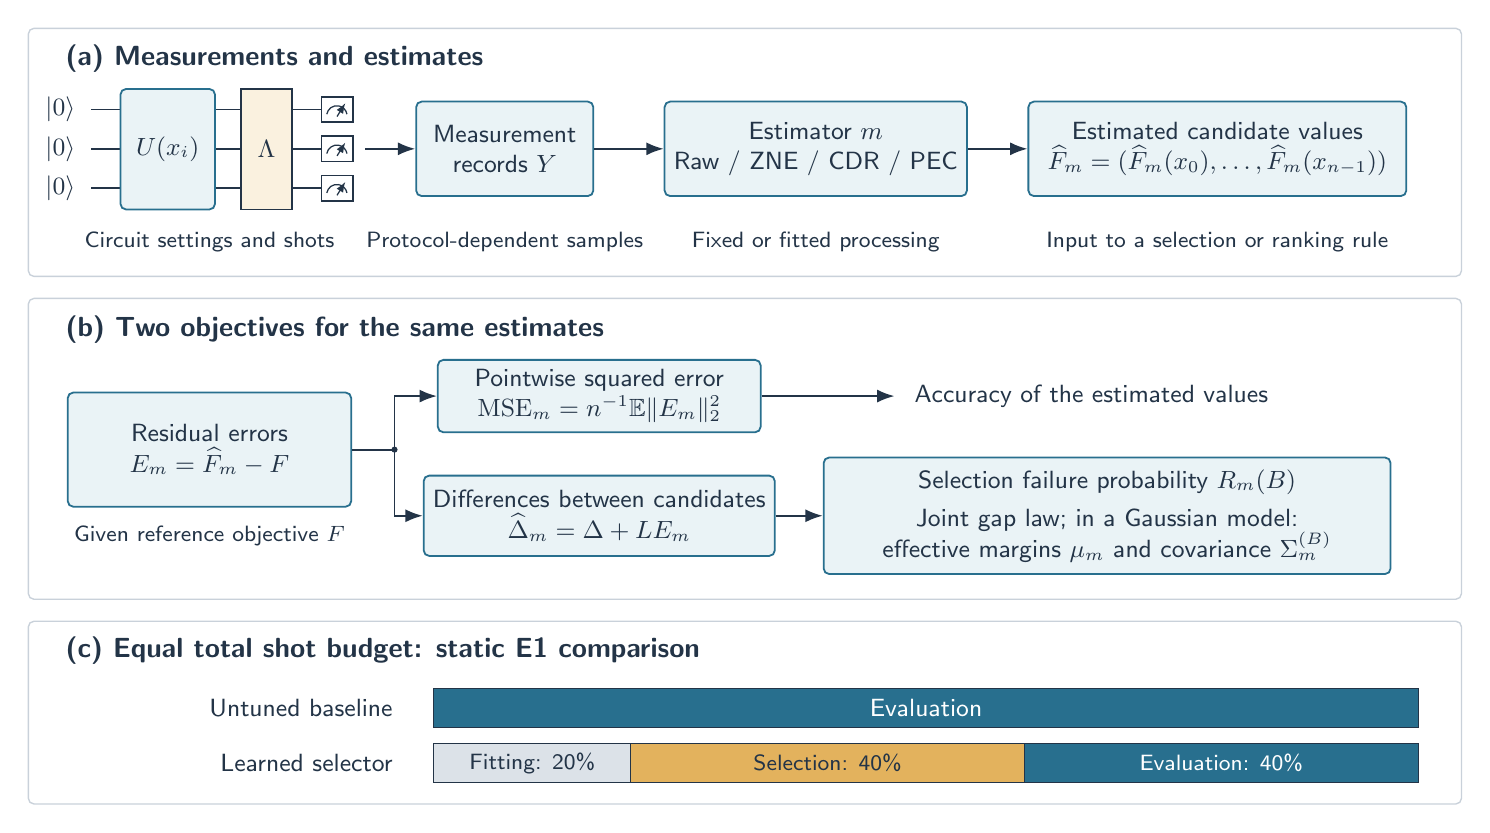
\begin{tikzpicture}[x=1cm,y=1cm,text=ink,
  font=\sffamily\fontsize{9}{11}\selectfont,
  flow/.style={-{Latex[length=2.2mm]},draw=ink,line width=.7pt},
  panel/.style={draw=border,fill=white,rounded corners=2pt,line width=.5pt},
  box/.style={draw=blue,fill=pale,rounded corners=2pt,line width=.65pt,align=center},
  head/.style={anchor=west,font=\sffamily\bfseries\fontsize{10}{12}\selectfont},
  small/.style={font=\sffamily\fontsize{8}{10}\selectfont,align=center}]

% (a) Physical records and estimates. The circuit is schematic.
\draw[panel] (0,6.70) rectangle (18.2,9.85);
\node[head] at (.35,9.47) {(a) Measurements and estimates};
\foreach \y in {8.82,8.32,7.82}{
  \node[anchor=east] at (.72,\y) {$|0\rangle$};
  \draw[ink,line width=.6pt] (.80,\y)--(4.13,\y);
}
\draw[box] (1.17,7.55) rectangle (2.37,9.08);
\node at (1.77,8.32) {$U(x_i)$};
\draw[draw=ink,fill=paleamber,line width=.6pt] (2.70,7.55) rectangle (3.35,9.08);
\node at (3.025,8.32) {$\Lambda$};
\foreach \y in {8.82,8.32,7.82}{\meter{3.92}{\y}}
\node[small] at (2.30,7.14) {Circuit settings and shots};

\node[box,minimum width=2.25cm,minimum height=1.20cm] (records) at (6.05,8.32)
 {Measurement\\records $Y$};
\draw[flow] (4.28,8.32)--(records.west);
\node[small] at (6.05,7.14) {Protocol-dependent samples};

\node[box,minimum width=3.4cm,minimum height=1.20cm] (method) at (10.0,8.32)
 {Estimator $m$\\\small Raw / ZNE / CDR / PEC};
\draw[flow] (records.east)--(method.west);
\node[small] at (10.0,7.14) {Fixed or fitted processing};

\node[box,minimum width=4.8cm,minimum height=1.20cm] (est) at (15.10,8.32)
 {Estimated candidate values\\$\widehat F_m=(\widehat F_m(x_0),\ldots,\widehat F_m(x_{n-1}))$};
\draw[flow] (method.east)--(est.west);
\node[small] at (15.1,7.14) {Input to a selection or ranking rule};

% (b) Two objectives. Ideal reference information is explicit.
\draw[panel] (0,2.60) rectangle (18.2,6.42);
\node[head] at (.35,6.03) {(b) Two objectives for the same estimates};
\node[box,minimum width=3.6cm,minimum height=1.45cm] (err) at (2.30,4.50)
 {Residual errors\\$E_m=\widehat F_m-F$};
\node[small] at (2.30,3.40) {Given reference objective $F$};

\node[box,minimum width=4.1cm,minimum height=.90cm] (mse) at (7.25,5.18)
 {Pointwise squared error\\$\mathrm{MSE}_m=n^{-1}\mathbb E\|E_m\|_2^2$};
\node[box,minimum width=4.1cm,minimum height=1.02cm] (gaps) at (7.25,3.66)
 {Differences between candidates\\$\widehat\Delta_m=\Delta+LE_m$};
\draw[flow] (err.east)--(4.65,4.50)|-(mse.west);
\draw[flow] (4.65,4.50)|-(gaps.west);
\fill[ink] (4.65,4.50) circle (1.1pt);

\node[align=center] (accuracy) at (13.50,5.18)
 {Accuracy of the estimated values};
\draw[flow] (mse.east)--(11.0,5.18);

\node[box,minimum width=7.2cm,minimum height=1.48cm] (risk) at (13.70,3.66)
 {Selection failure probability $R_m(B)$\\[3pt]
  \small Joint gap law; in a Gaussian model:\\
  \small effective margins $\mu_m$ and covariance $\Sigma_m^{(B)}$};
\draw[flow] (gaps.east)--(risk.west);

% (c) Actual normalized acquisition shares of the static E1 comparison.
\draw[panel] (0,0) rectangle (18.2,2.32);
\node[head] at (.35,1.95) {(c) Equal total shot budget: static E1 comparison};
\node[anchor=east] at (4.75,1.22) {Untuned baseline};
\node[anchor=east] at (4.75,.52) {Learned selector};
\draw[fill=blue,draw=ink,line width=.4pt] (5.15,.97) rectangle (17.65,1.47);
\node[text=white] at (11.40,1.22) {Evaluation};
\draw[fill=gray,draw=ink,line width=.4pt] (5.15,.27) rectangle (7.65,.77);
\draw[fill=amber,draw=ink,line width=.4pt] (7.65,.27) rectangle (12.65,.77);
\draw[fill=blue,draw=ink,line width=.4pt] (12.65,.27) rectangle (17.65,.77);
\node[small] at (6.40,.52) {Fitting: 20\%};
\node[small] at (10.15,.52) {Selection: 40\%};
\node[small,text=white] at (15.15,.52) {Evaluation: 40\%};
\end{tikzpicture}
\end{document}
